%\documentclass[]{beamer}
%\documentclass[handout]{beamer}
\documentclass[handout,draft]{beamer}

% Preambulo
% Paquetes para usar bien el idioma español
\usepackage[spanish,es-tabla]{babel}
\selectlanguage{spanish}
\usepackage[utf8]{inputenc}

% Paquetes para usar mejores imagenes
\usepackage{graphicx}

% Paquetes para links y tabla de contenidos en el PDF
\usepackage{hyperref}
\hypersetup{colorlinks=true,allcolors=blue}
%\usepackage{hypcap}

% Paquetes para mejores tablas
\usepackage{booktabs}

% Mejor matematica
\usepackage{amsmath}

% Fuentes de las imagenes
\usepackage[absolute,overlay]{textpos}

% Paquete captions
\usepackage[justification=centering,labelformat=empty,labelsep=none]{caption}

% Opciones para ticks
\usepackage{tikz}
\usetikzlibrary{shapes,arrows,positioning}

\tikzstyle{decision} = [diamond, draw, fill=blue!20, text width=4em, text badly centered, node distance=2cm, inner sep=0pt,on grid]
\tikzstyle{block} = [rectangle, draw, fill=blue!20, text width=8em, text centered, rounded corners, minimum height=2em,on grid]
\tikzstyle{line} = [draw, -latex]

% Citas bibliograficas
\usepackage[backend=biber]{biblatex}
\renewcommand{\footnotesize}{\tiny}
\addbibresource{biblio.bib}

% Mejoro las captions
\setbeamertemplate{caption}{\raggedright\insertcaption\par}

\setbeamertemplate{caption}{%
\begin{beamercolorbox}[wd=0.85\paperwidth, sep=.2ex]{block body}\insertcaption%
\end{beamercolorbox}%
}


% Sacar barra de navegacion
\setbeamertemplate{navigation symbols}{}%remove navigation symbols

% Transparencias en items
\setbeamercovered{transparent}

% Estilo de diapositivas
% \usetheme{Boadilla}
\usecolortheme{whale}
\usecolortheme{orchid}


\title{Herramientas de Teledetección Cuantitativa\\{\small Clase 1}}
\author{Francisco Nemi\~na}
\institute[Inst.]{
\includegraphics[height=1cm]{imagenes/logosopi.png}\phantom{pepe} 
\includegraphics[height=1cm]{imagenes/2mp.png}\phantom{pepe} 
\includegraphics[height=1cm]{imagenes/conae.png}}
\date{}
%\titlegraphic{
%\includegraphics[height=1cm]{imagenes/minplan.png}\phantom{1}
%
\includegraphics[height=1cm]{imagenes/conae.png}\phantom{1}
%
\includegraphics[height=1cm]{imagenes/sopi.png}}

\logo{
\includegraphics[height=0.7cm]{imagenes/sopi.png}}

\AtBeginSection[]
{
\begin{frame}
\frametitle{Esquema de presentaci\'on}
\tableofcontents[currentsection]
\end{frame}
}

\begin{document}
\begin{frame}
    \maketitle
\end{frame}

\section{Introducción}
\subsection{Organización del curso}
\begin{frame}
  \frametitle{Objetivos del curso}
  \begin{itemize}
    \item<1-> Poder analizar en detalle una {\only<|2->{\color{red}}firma espectral.}
    \item<2> Familiarizarse con el concepto de reflectancia bidireccional.
    \item<3> Conocer las distintas fuentes de distorsión radiométrica.
    \item<4> Comprender el concepto de dimensionalidad y como reducir la misma.
    \item<5> Poder realizar clasificaciones supervisadas y no supervisadas comprendiendo los fundamentos matemáticos detrás de las mismas.
    \item<6> Poder realizar validaciones de clasificaciones.
    \item<7> Realizar estudios de series temporales.
  \end{itemize}
\end{frame}

\begin{frame}[fragile]{Organizaci\'on del curso}
  \begin{block}{Plataforma de Educaci\'on a Distancia}
    \verb+https://sopi.conae.gov.ar/aulavirtual+\\
    \verb+Contraseña: sopiII2015+
  \end{block}\pause
  \begin{block}{Aprobaci\'on}
    \begin{enumerate}
      \item 75\% de asistencia.
      \item 7 cuestionarios te\'orico-pr\'acticos sobre las clases
      \item 1 trabajo final integrador
    \end{enumerate}\pause
  \end{block}
  \begin{alertblock}{Modalidad de trabajo}
    Te\'orico-pr\'actico con la inclusión de lecturas complementarias.
  \end{alertblock}
\end{frame}
%--- Next Frame ---%

\begin{frame}[fragile]{Organizaci\'on del curso}
  \begin{block}{Cronograma}
    \begin{itemize}[<+>]
      \item 18/9 - Conceptos b\'asicos y firmas espectrales.
      \item 25/9 - Correcciones radiom\'etricas.
      \item 2/10 - Dimensionalidad e \'indices.
      \item 9/10 - Clasificaciones no supervisadas.
      \item 16/10 - Clasificaciones supervisadas.
      \item 23/10 - Clase de consulta.
      \item 30/10 - Validaci\'on de datos satelitales.
      \item 6/11 - Detecci\'on de cambios.
      \item 13/11 - Clase de consulta.
      \item 20/11 - Entrega del trabajo final.
    \end{itemize}
  \end{block}
\end{frame}

\begin{frame}{M\'etodos cuantitativos}
  \begin{block}{Definici\'on:}
    Hablamos de \emph{m\'etodos cuantitativos en teledetecci\'on \'optica} cuando queremos cuantificar los datos disponibles en una imagen para poder extraer informaci\'on de las mismas utilizando las longitudes de onda de $0.4\mu m$ a $14 \mu m$.
  \end{block}
\end{frame}
%--- Next Frame ---%

\begin{frame}{M\'etodos cuantitativos}
  \begin{enumerate}
    \item<1-3> Tipos de modelos
    \begin{enumerate}
      \item<2-3> estad\'isticos
      \item<3> biofísicos
    \end{enumerate}
    \item<4-6> Tipos de variables
    \begin{enumerate}
      \item<5-6> continuas
      \item<6> categ\'oricas
    \end{enumerate}
  \end{enumerate}
\end{frame}
%--- Next Frame ---%

\section{Conceptos b\'asicos}
\subsection{Radiancia}
\begin{frame}{Radiancia}
  \begin{block}{Definici\'on:}
    $$dE = L_{\lambda}(\theta,\phi) \cos(\theta) d\Omega dA dt d\lambda$$
    Potencia radiante por unidades de \'area y \'angulo s\'olido.
  \end{block}\pause
  \begin{alertblock}{Importante:}
    \begin{itemize}[<+>]
      \item $[L_{\lambda}] = \frac{W}{m^2 sr nm}$
      \item Es una de las dos magnitudes m\'as relevantes.
    \end{itemize}
  \end{alertblock}
\end{frame}
%--- Next Frame ---%

\begin{frame}{Radiancia}
  \begin{figure}
  \centering
  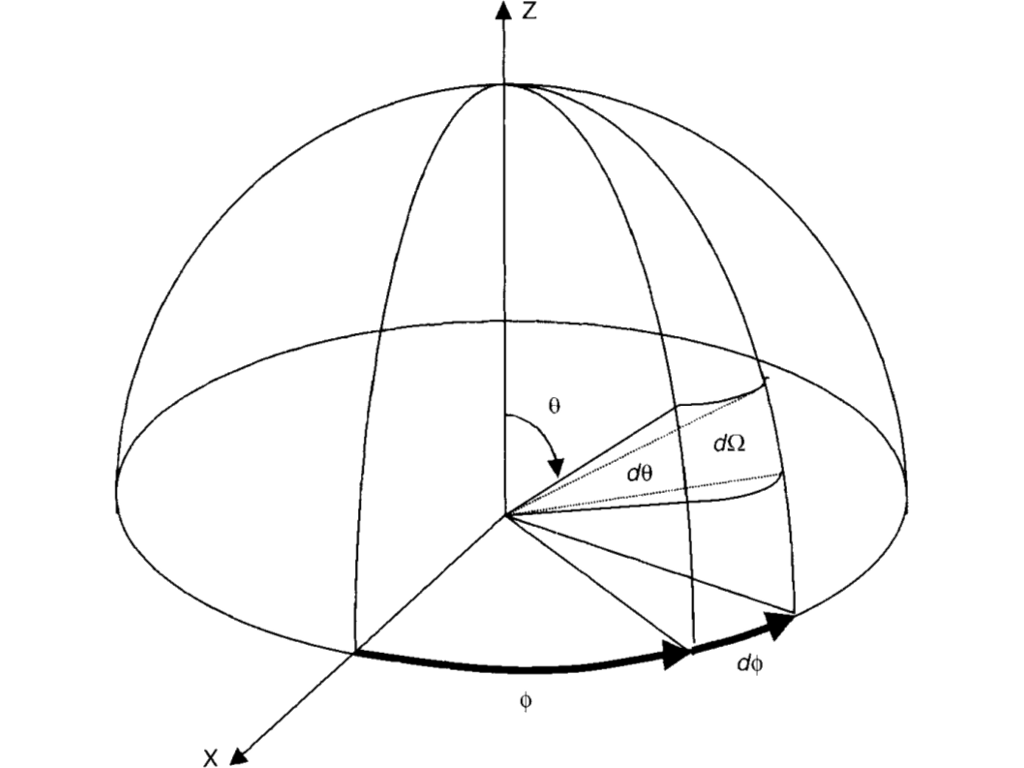
\includegraphics[width=0.8\textwidth]{imagenes/solid_angle.png}
  \caption{\'Angulo s\'olido $\Omega$ y los \'angulos asociados $\theta$ y $\phi$.\footfullcite{liang2005quantitative}}
  \end{figure}
\end{frame}
%--- Next Frame ---%

\begin{frame}{Radiancia}
  \begin{block}{Definici\'on}
    Definimos la irradiancia como
    $$E=\int L(\theta,\phi) \cos(\theta) d\Omega$$\pause
    para el caso de que la luz se emita s\'olo en uno de los hemisferios
    $$E=\int_0^{2\pi}\int_0^{\pi/2} L(\theta,\phi) \cos(\theta) \sin(\theta) d\theta d\phi$$
  \end{block}
\end{frame}
%--- Next Frame ---%

\begin{frame}{Radiancia}
  \begin{figure}
  \centering
  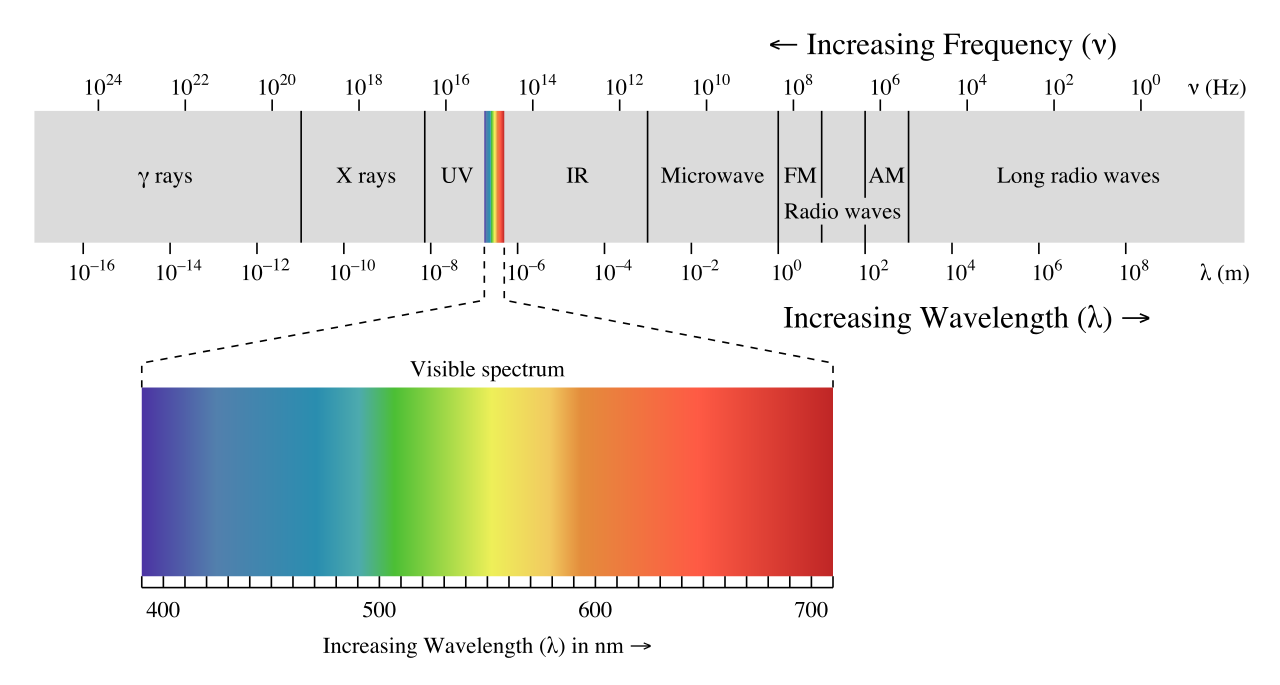
\includegraphics[width=0.8\textwidth]{imagenes/espectrum.png}
  \caption{Espectro electromagn\'etico.\footfullcite{espectrum}}
  \end{figure}
\end{frame}
%--- Next Frame ---%

\begin{frame}{Radiancia}
  \begin{figure}
  \centering
  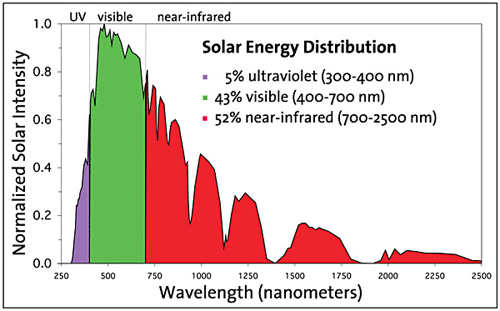
\includegraphics[width=0.8\textwidth]{imagenes/blackpercent.png}
  \caption{Irradiancia medida sobre la superficie terrestre.\footfullcite{blackpercent}}
  \end{figure}
\end{frame}
%--- Next Frame ---%

\begin{frame}{Radiancia}
  \begin{block}{Curva de irradiancia}
    C\'alculo de la irradiancia de un cuerpo negro
    $$ L(\lambda,T) = \frac{2hc^2}{\lambda^5}\frac{1}{e^{\frac{hc}{\lambda k_B T}}-1}$$
  \end{block}
\end{frame}
%--- Next Frame ---%

\begin{frame}{Radiancia}
  \begin{figure}
  \centering
  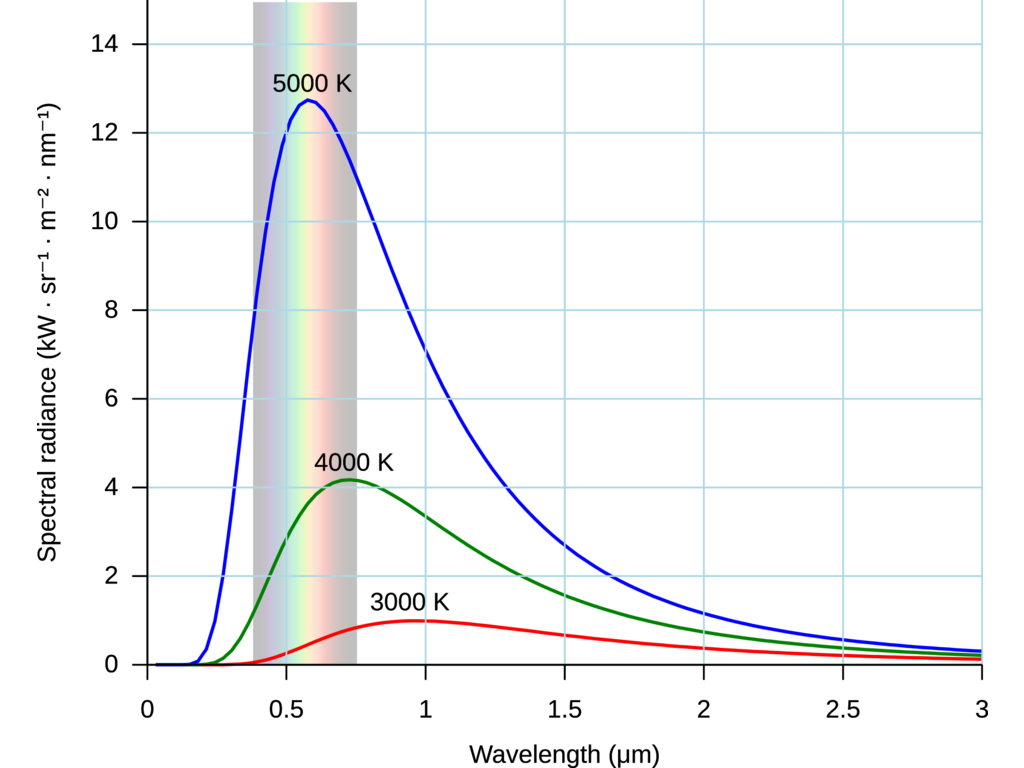
\includegraphics[width=0.8\textwidth]{imagenes/blackbody.png}
  \caption{Curva de irradiancia para un cuerpo negro.\footfullcite{blackbody}}
  \end{figure}
\end{frame}
%--- Next Frame ---%

\begin{frame}{Radiancia}
  \begin{block}{C\'alculo de la irradiancia solar}
    C\'alculo de la irradiancia solar
    $$S_0 = \int_0^\infty E_0(\lambda) d\lambda$$
    su valor aproximado es
    $$ S_0 = 1369 W/m^2$$
    \pause es la cantidad de luz que llega del sol.
  \end{block}
\end{frame}
%--- Next Frame ---%

\begin{frame}{Valores tipos de L}
  \begin{exampleblock}{Valores tipos de E para Landsat}
    En $[L_{\lambda}] = \frac{W}{m^2 \mu m}$
    \begin{figure}
      \begin{tabular}{l c c}
        Banda & ETM+  & TM    \\
        1     & 1970  & 1954  \\
        2     & 1843  & 1826  \\
        3     & 1555  & 1558  \\
        4     & 1047  & 1047  \\
        5     & 227.1 & 217.2 \\
        7     & 80.53 & 80.29 \\
      \end{tabular}
    \end{figure}
  \end{exampleblock}
\end{frame}
%--- Next Frame ---%

\subsection{Reflectancia}

\begin{frame}{Reflectancia}
  \begin{figure}
  \centering
  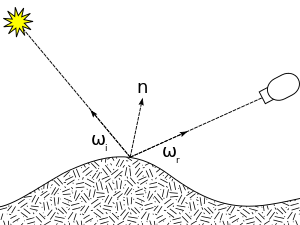
\includegraphics[width=0.8\textwidth]{imagenes/brdf.png}
  \caption{Irradiancia incidente y reflejada por una cobertura.\footfullcite{brdf}}
  \end{figure}
\end{frame}
%--- Next Frame ---%

\begin{frame}{Reflectancia}
  \begin{block}{Definici\'on:}
    Definimos la BRDF (espectral bidirectional reflectance distribution function) como:
    $$ f(\theta_i, \phi_i, \theta_r, \phi_r) = \frac{dL(\theta_i, \phi_i, \theta_r, \phi_r)}{dE(\theta_i, \phi_i)}$$
  \end{block}
  \pause
  \begin{block}{Definici\'on:}
    Defininimos la reflectancia direccional como:
    $$ R(\theta_i, \phi_i, \theta_r, \phi_r) = \frac{\pi L(\theta_i, \phi_i, \theta_r, \phi_r)}{\cos(\theta_i) E_0} = \pi f(\theta_i, \phi_i, \theta_r, \phi_r)$$
  \end{block}
\end{frame}
%--- Next Frame ---%

\begin{frame}{Reflectancia}
  \begin{figure}
  \centering
  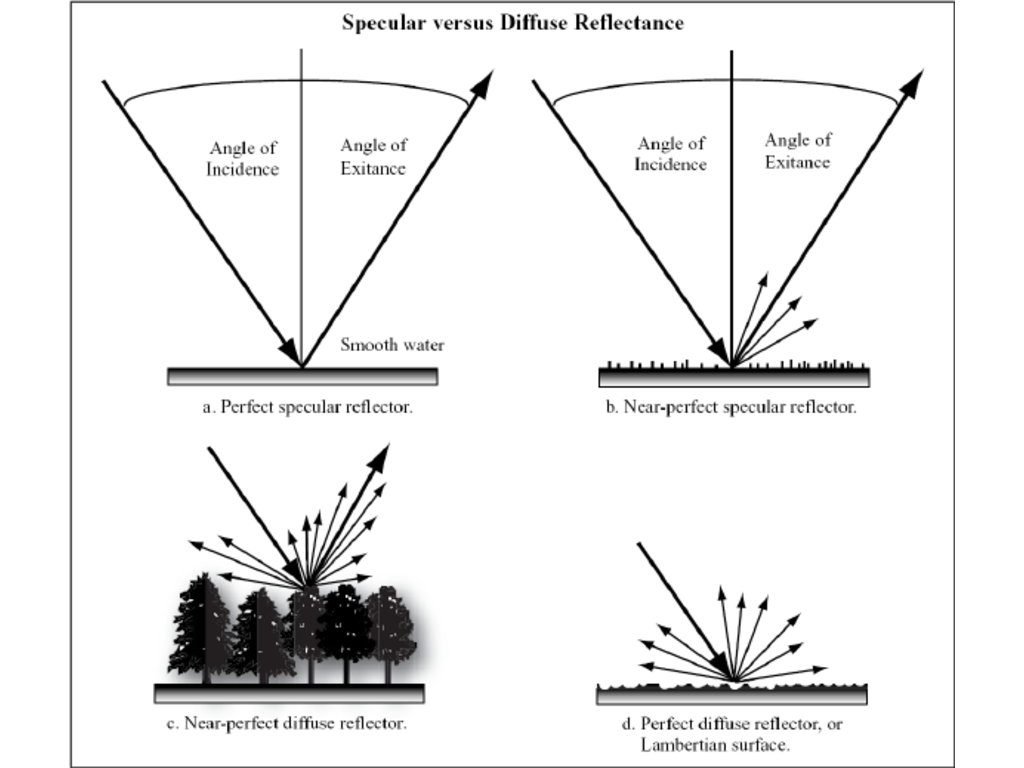
\includegraphics[width=0.8\textwidth]{imagenes/difusa.png}
  \caption{Distintos casos de reflectancia direccional.\footfullcite{jensen2007remote}}
  \end{figure}
\end{frame}
%--- Next Frame ---%

\begin{frame}{Reflectancia}
  \begin{block}{Aproximaci\'on lambertiana}
    Hablamos de la aproximaci\'on lambertiana cuando la reflectancia no depende del \'angulo reflejado
    $$\rho = \frac{\pi L}{\mu_i E_0}$$
    donde tomamos $\mu=cos(\theta)$
  \end{block}
\end{frame}
%--- Next Frame ---%

\section{Firma espectral}
\subsection{Medici\'on}
\begin{frame}{Medici\'on}
  \begin{block}{Definici\'on:}
    La distribuci\'on de la reflectancia es funci\'on de la longitud de onda nos habla de la caracter\'isticas intr\'insecas de la cobertura. Es su firma espectral $\rho_\lambda$.
  \end{block}
\end{frame}
%--- Next Frame ---%

\begin{frame}{Medici\'on}
  \begin{block}{Respuesta espectral}
    Podemos pensar a la respuesta de un sensor como una integral
      $$\rho_{j} =\frac{\int s_j(\lambda) \rho d\lambda}{\int s_j(\lambda) d\lambda}$$
    donde si pensamos a la respuesta como una distribuci\'on podemos definir $\lambda_c$ y $\Delta \lambda$ el centro de la adquisici\'on y ancho de banda efectivo.
  \end{block}\pause
  \begin{alertblock}{Importante}
    Desde el punto de vista espectral, las resoluciones espectral y radiom\'etrica, nos permiten distinguir distintas cosas de la firma espectral.
  \end{alertblock}
\end{frame}
%--- Next Frame ---%

\begin{frame}{Medici\'on}
  \begin{figure}\centering
    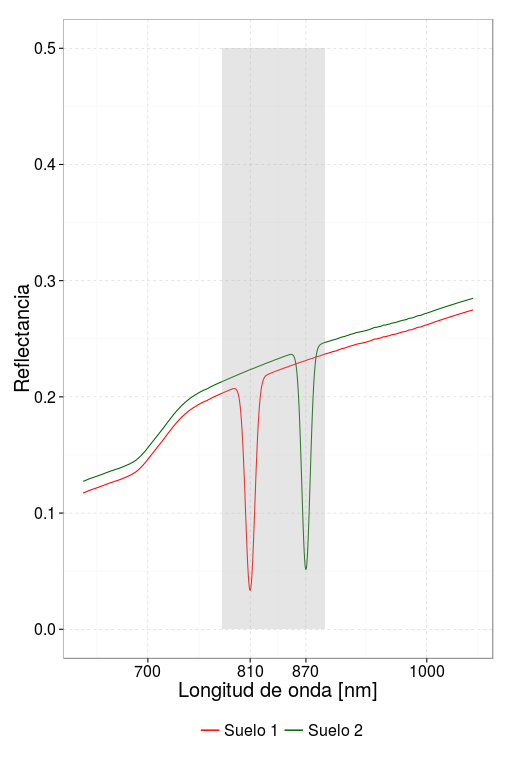
\includegraphics[width=0.4\textwidth]{imagenes/ebaja.png}\phantom{F}
    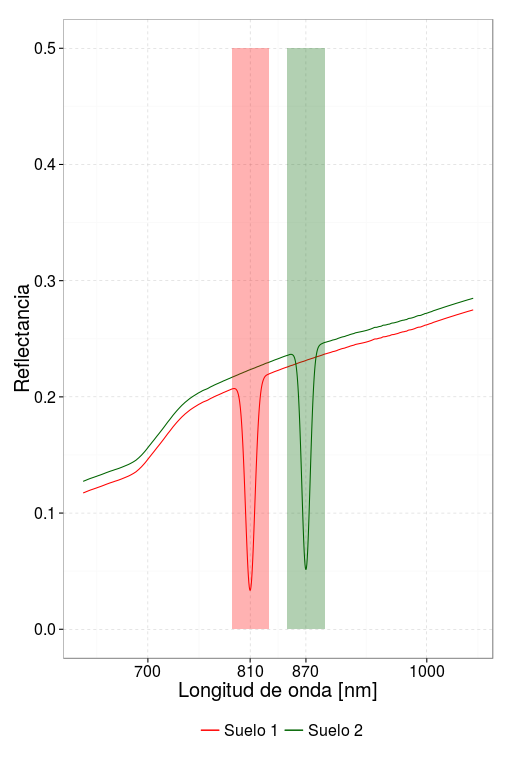
\includegraphics[width=0.4\textwidth]{imagenes/ealta.png}
    \caption{Espectral separa.}
  \end{figure}
\end{frame}
%--- Next Frame ---%

\begin{frame}{Medici\'on}
  \begin{figure}\centering
    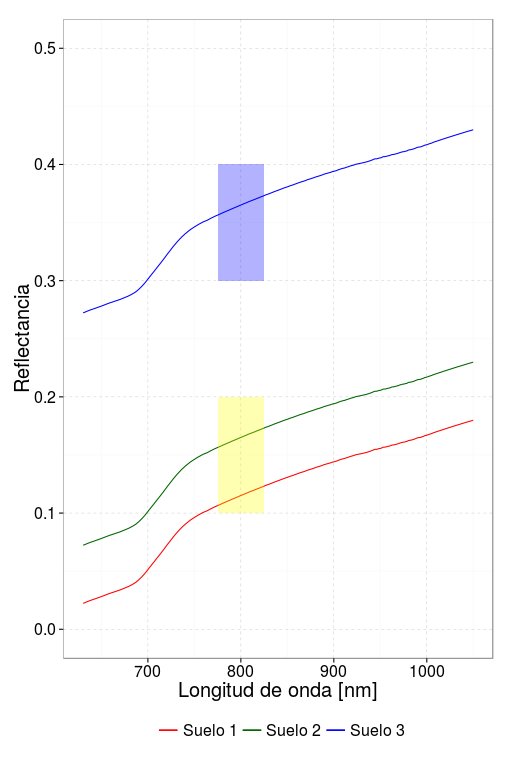
\includegraphics[width=0.4\textwidth]{imagenes/rbaja.png}\phantom{F}
    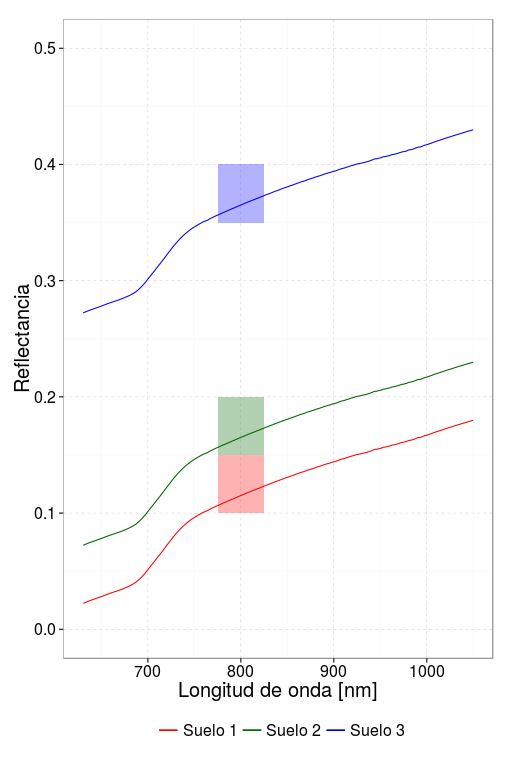
\includegraphics[width=0.4\textwidth]{imagenes/ralta.png}
    \caption{Resoluci\'on radiom\'etrica.}
  \end{figure}
\end{frame}
%--- Next Frame ---%

\begin{frame}{Medici\'on}
  \begin{figure}
  \centering
  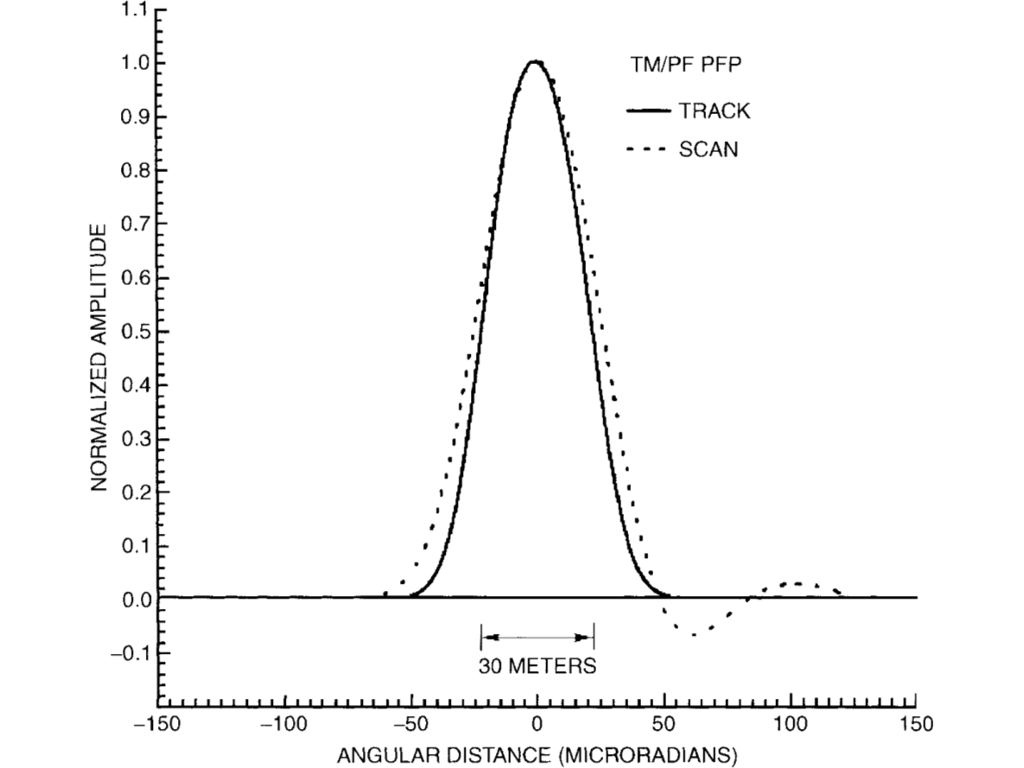
\includegraphics[width=0.8\textwidth]{imagenes/respacial.png}
  \caption{Respuesta espacial de un sensor en ambas direcciones.\footfullcite{liang2005quantitative}}
  \end{figure}
\end{frame}
%--- Next Frame ---%

\begin{frame}{Medici\'on}
  \begin{block}{Respuesta espacial}
    \begin{itemize}
      \item La resoluci\'on espacial sale de esta funci\'on.
      \item Es importante por que nos permite comprender la formaci\'on de un p\'ixel.
    \end{itemize}
  \end{block}
  \begin{block}{Formaci\'on de un p\'ixel}
    El valor de reflectancia para un p\'ixel vale
    $$\rho_{pix} = \sum_i w_i \rho_i$$
    donde $w_i$ corresponde a la distinta cobertura de cada p\'ixel.
  \end{block}
\end{frame}

\subsection{Modelado}

\begin{frame}{Modelado}
  \begin{figure}
  \centering
  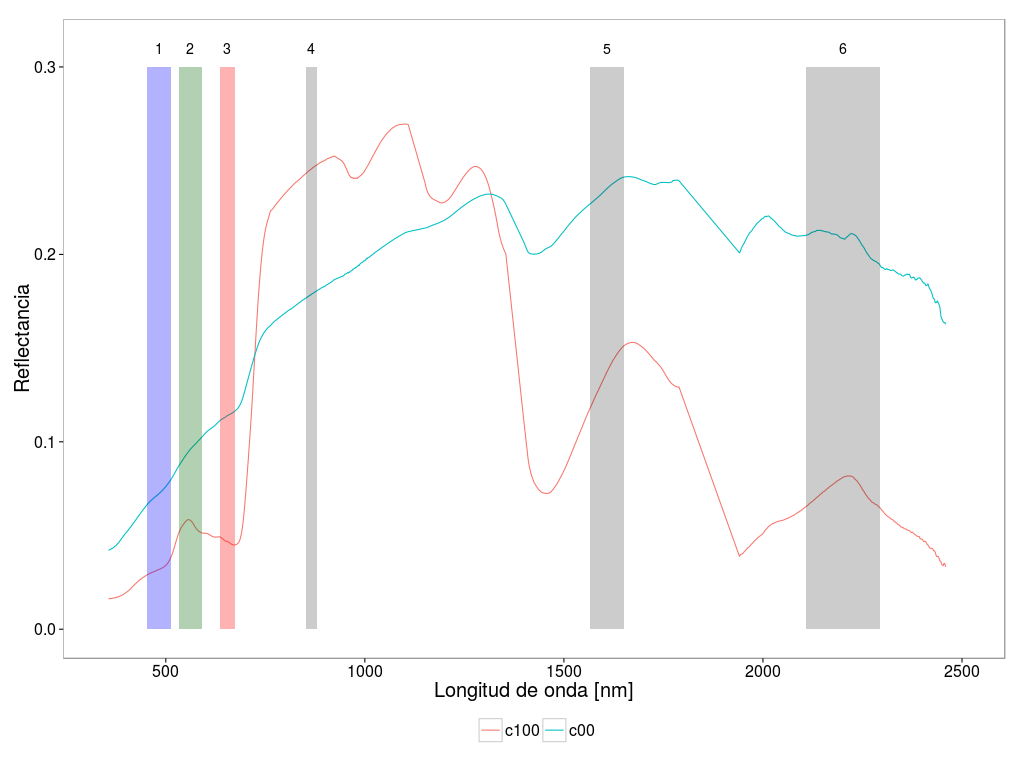
\includegraphics[width=0.8\textwidth]{imagenes/puras.png}
  \caption{Firmas espectrales de vegetaci\'on y suelo desnudo.\footfullcite{clark2007usgs}}
  \end{figure}
\end{frame}
%--- Next Frame ---%

\begin{frame}{Modelado}
  \begin{figure}
  \centering
  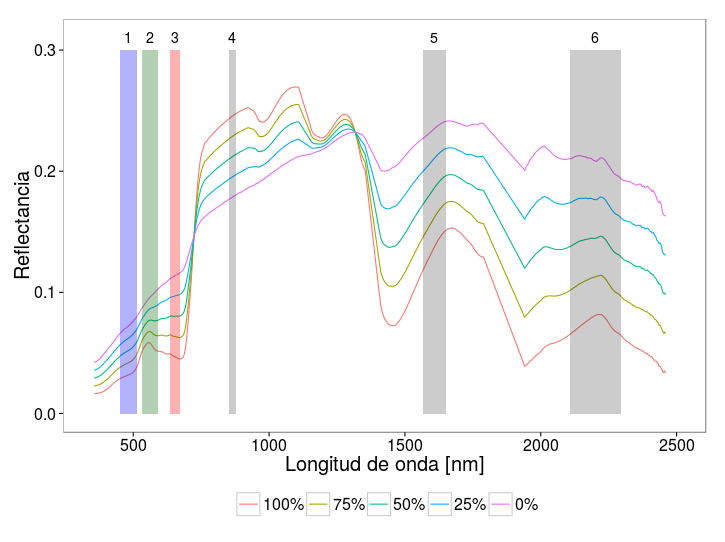
\includegraphics[width=0.8\textwidth]{imagenes/mezcla.png}
  \caption{Mezcla de firmas espectrales para un gradiente de coberturas.\footfullcite{clark2007usgs}}
  \end{figure}
\end{frame}
%--- Next Frame ---%

\begin{frame}{Modelado}
  La vegetaci\'on tiene 3 zonas del espectro principales que modelar
  \begin{itemize}
    \item<1> Visible
    \item<2> Infrarrojo cercano
    \item<3> Infrarrojo de onda media
  \end{itemize}
\end{frame}
%--- Next Frame ---%

\begin{frame}{Modelado}
    \begin{figure}
    \centering
    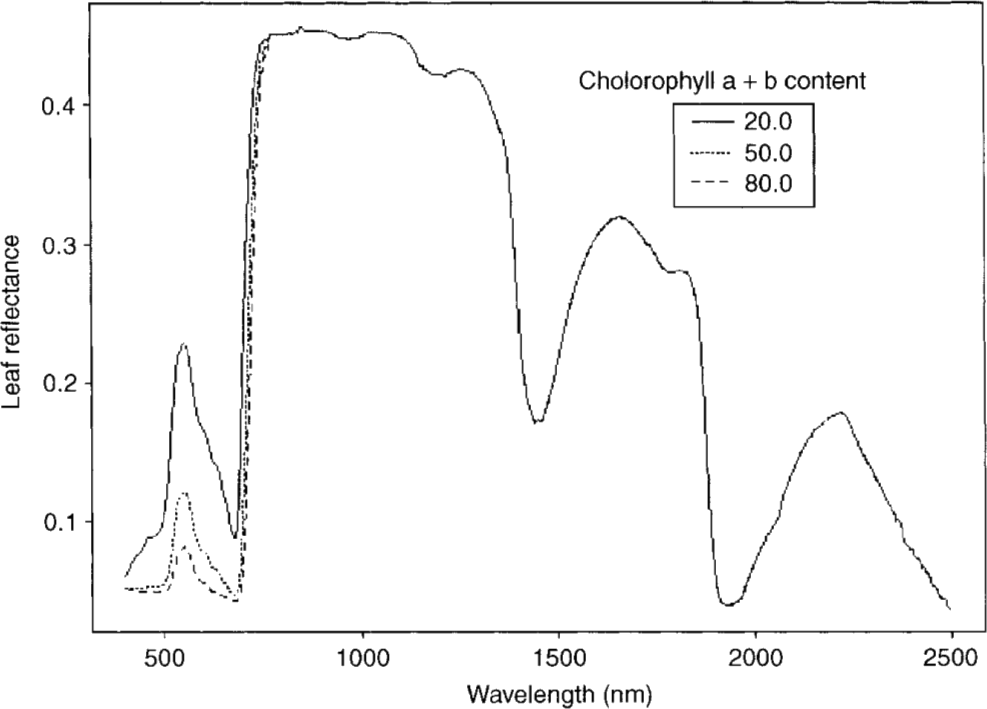
\includegraphics[width=0.8\textwidth]{imagenes/clorovar.png}
    \caption{Variaciones de la firma espectral con el contenido de clorofila.\footfullcite{liang2005quantitative}}
    \end{figure}
\end{frame}
%--- Next Frame ---%

\begin{frame}{Modelado}
    \begin{figure}
    \centering
    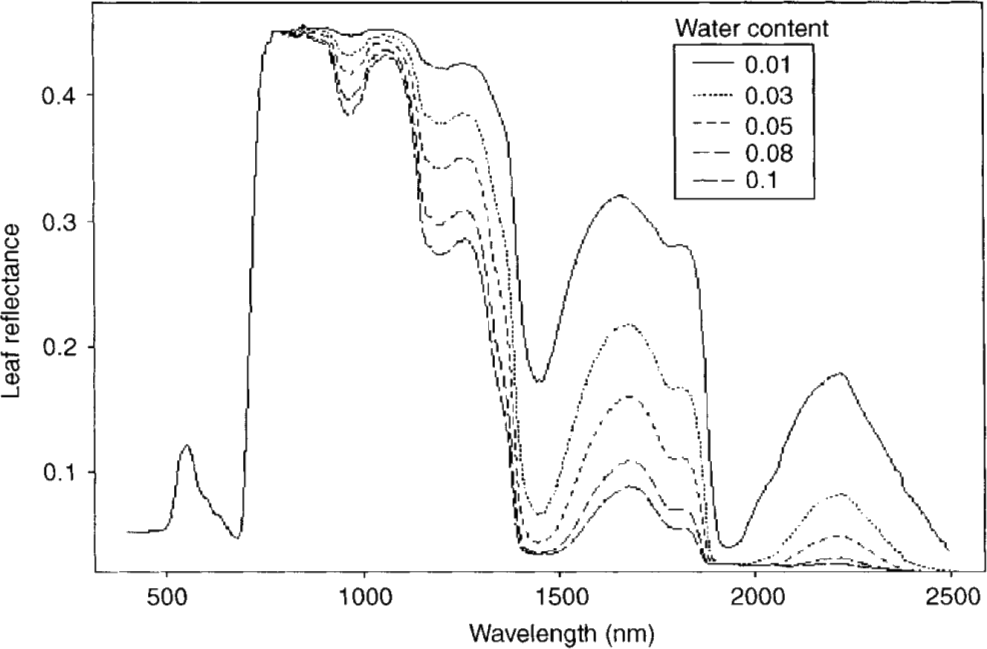
\includegraphics[width=0.8\textwidth]{imagenes/vwvar.png}
    \caption{Variaciones de la firma espectral con el contenido de agua.\footfullcite{liang2005quantitative}}
    \end{figure}
\end{frame}
%--- Next Frame ---%

\begin{frame}{Modelado}
    \begin{figure}
    \centering
    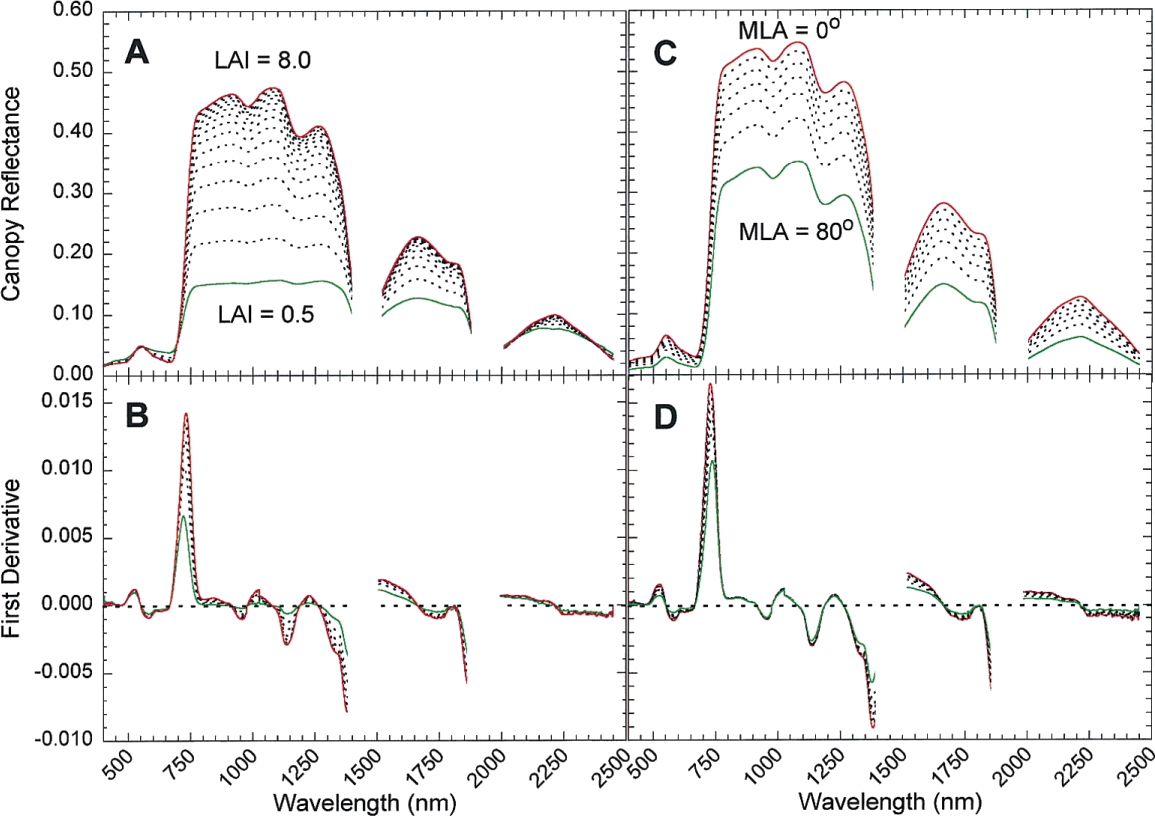
\includegraphics[width=0.8\textwidth]{imagenes/leafvar.png}
    \caption{Variaciones de la firma espectral con el \'area foliar.\footfullcite{asner1998biophysical}}
    \end{figure}
\end{frame}
%--- Next Frame ---%

\begin{frame}{Modelado}
    \begin{figure}
    \centering
    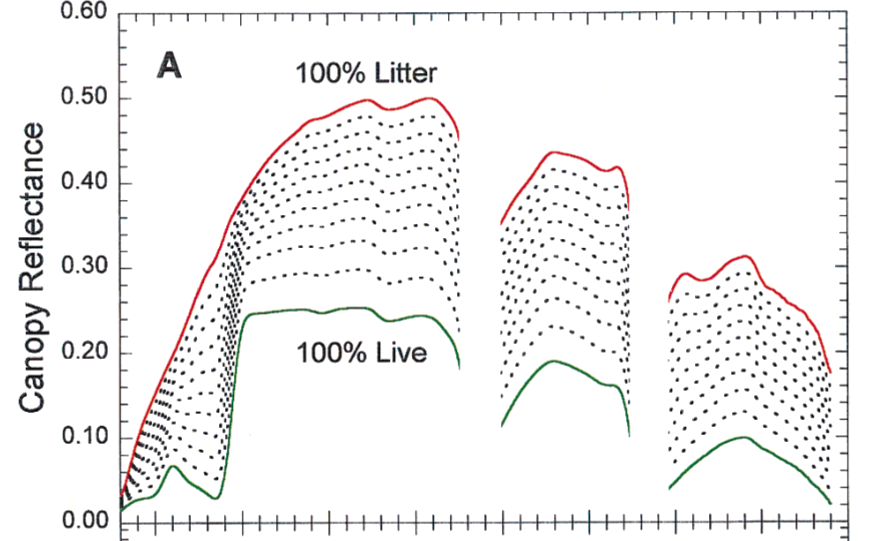
\includegraphics[width=0.8\textwidth]{imagenes/vivomuerto.png}
    \caption{Firma espectral de la vegetación en diferentes estados.\footfullcite{asner1998biophysical}}
    \end{figure}
\end{frame}
%--- Next Frame ---%

\begin{frame}{Modelado}
    \begin{figure}
    \centering
    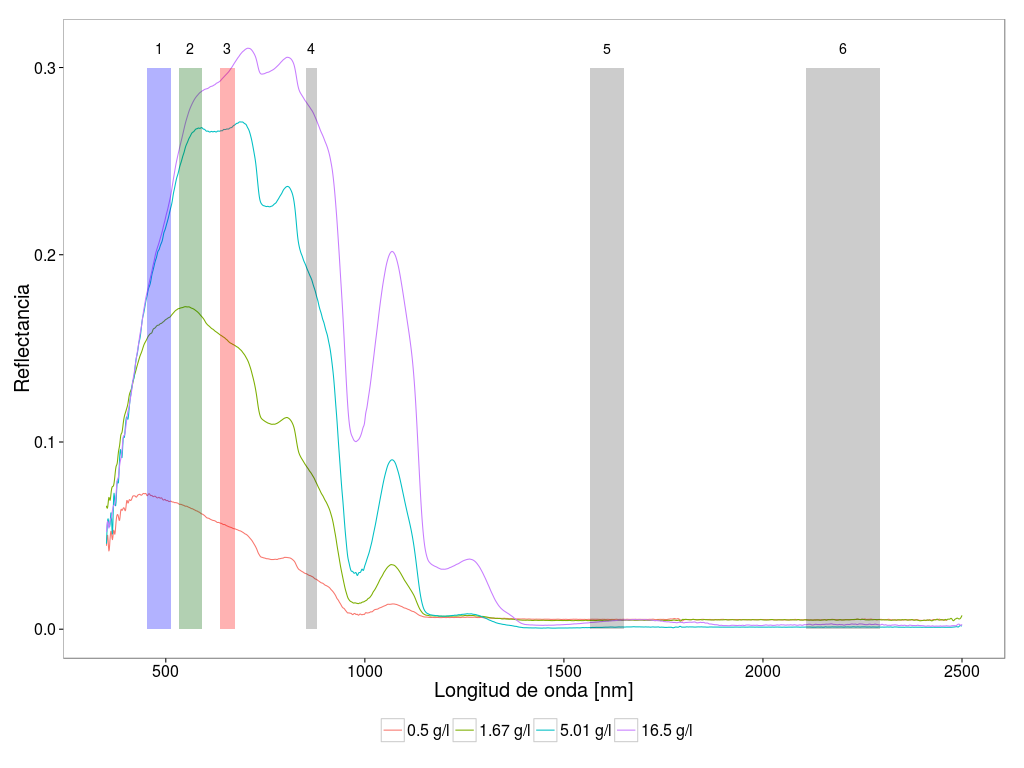
\includegraphics[width=0.8\textwidth]{imagenes/waterm.png}
    \caption{Firma espectral de agua con distinto contenido de arcilla disuelta.\footfullcite{clark2007usgs}}
    \end{figure}
\end{frame}
%--- Next Frame ---%

\begin{frame}{Modelado}
    \begin{figure}
    \centering
    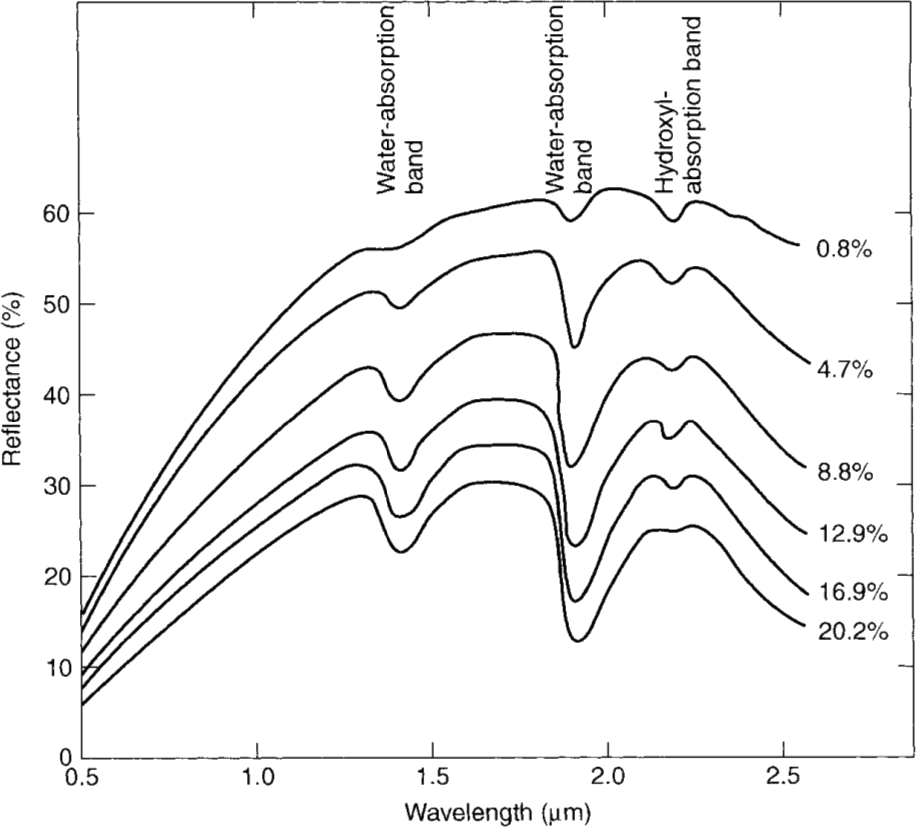
\includegraphics[width=0.6\textwidth]{imagenes/soilvar.png}
    \caption{Firma espectral del suelo con distintos contenidos de humedad.\footfullcite{liang2005quantitative}}
    \end{figure}
\end{frame}
%--- Next Frame ---%

\section{Pr\'actica}

\begin{frame}{Pr\'actica}
  \begin{exampleblock}{Actividades pr\'acticas de la primera clase}
    \begin{enumerate}
      \item Abrir im\'agenes Landsat 8 y familiarizarse con el SoPI.
      \item Digitalizar coberturas uniformes dentro de la imagen.
      \item Extraer la firma espectral de las coberturas digitalizadas.
      \item Reescalar las firmas obtenidas y compararlas para dos im\'agenes distintas.
    \end{enumerate}
  \end{exampleblock}
\end{frame}
%--- Next Frame ---%

\end{document}
